\chapter{Informationsbeschaffung}
\label{chap:Informationsbeschaffung}
Dieses Kapitel bietet fundamentale physikalische Gegebenheiten, sowie die relevanten Informationen über \ac{PIR} und verwendete 


\subsection*{Physikalische Grössen und Symbole}
\begin{table}[H]
	\begin{tabular}{l|c|c}
		
		\rowcolor{gray} Grösse &  Bezeichnung  & Einheit \\
		\hline 
		Wärmestrom &  $\dot{Q}$ & $J$  \\ 
		\rowcolor{gray}Emission & $\epsilon$ & $-$\\	
		Reflektion &  $\rho $ & $-$ \\
		\rowcolor{gray} Transmission & $\tau$ & $-$\\
		Absoprtion &  $\alpha$ & $-$  \\ 
		
		\rowcolor{gray}Geschwindigkeit des Chassis & $\dot{Q}$ & $m/s$\\
		Beschleunigung des Chassis &  a $\ddot{x}$ & $m/s^2$ \\
		\rowcolor{gray}Neigungswinkel des Chassis mit Balanciermasse &  $\varphi$ & rad \\ 
		Neigungswinkelgeschwindigkeit des Chassis mit Balanciermasse & $\dot\varphi $ & $ rad/s$ \\ 
		\rowcolor{gray} Neigungswinkelbeschleunigung des Chassis mit Balanciermasse & $\ddot\varphi $ & $ rad/s^2 $ \\ 
	\end{tabular}
	\caption{Legende physikalische Grössen Konzeptzeichnungen}
	\label{tab:Legende Physikalische Grössen} 
\end{table} 



\section{Physikalische Aspekte}

Die Physikalischen Grundlagen erläutert auf kurze und prägnante Weise die r

\begin{table}[]
	\centering
	\caption{Infrarotbereiche}
	\label{my-label}
	\begin{tabular}{|l|l|l|}
		\hline
		IR-A {[}$\mu$m{]} & IR-B {[}$\mu$m{]} & IR-C {[}$\mu$m{]} \\ \hline
		0.78 - 1.4  & 1.4 - 3.0   & 3 - 1000    \\ \hline
	\end{tabular}
\end{table}

\subsection{Allgemein}

\begin{equation}
\label{eq2}
\frac{\mathrm{d} Q}{\mathrm{d} t} = \epsilon *\sigma * A * T^4
\end{equation}
\myequations{Wärmestrahlung}

\begin{equation}
\label{eq1}
a^2+b^2=c^2
\end{equation}
\myequations{sum}


\subsection{Seebeck-Effekt}




\section{verwendete Sensorik}


\begin{figure}[H]
	\centering
	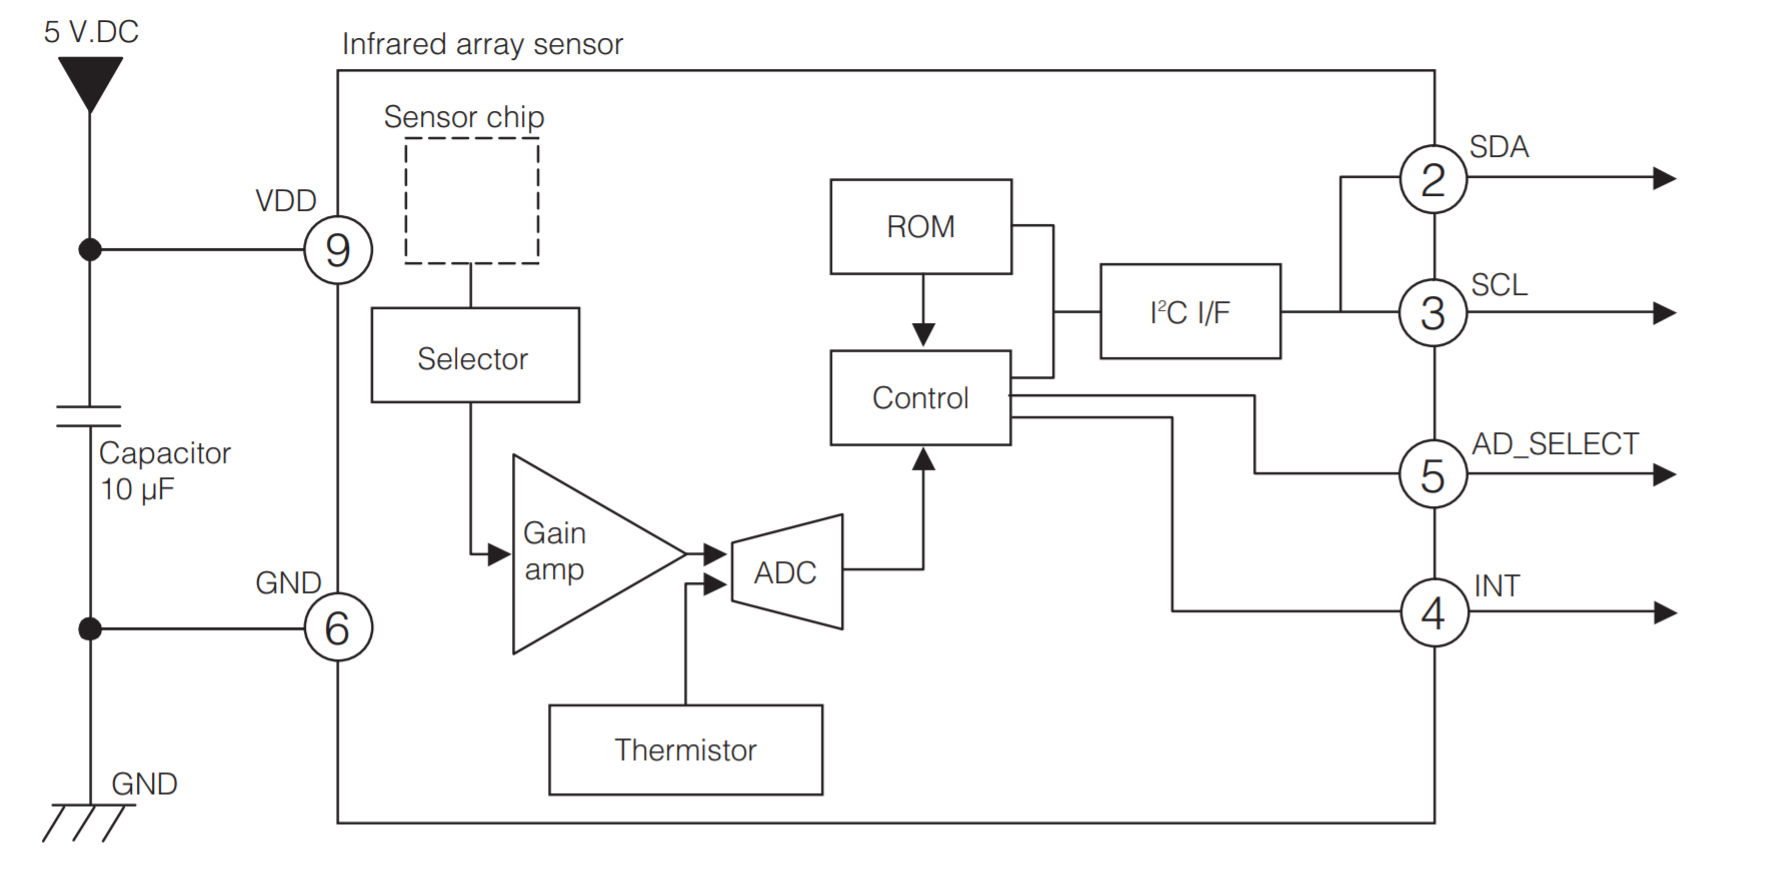
\includegraphics[width=0.8\textwidth]
	{fig/Circuit_AMG8834.PNG}
	\caption[Schema des AMG8834 Sensors]{Schema des AMG8834 Sensors} \protect\cite{AMG8834}
	\label{fig:angleVLP}
\end{figure}


\begin{figure}[H]
	\centering
	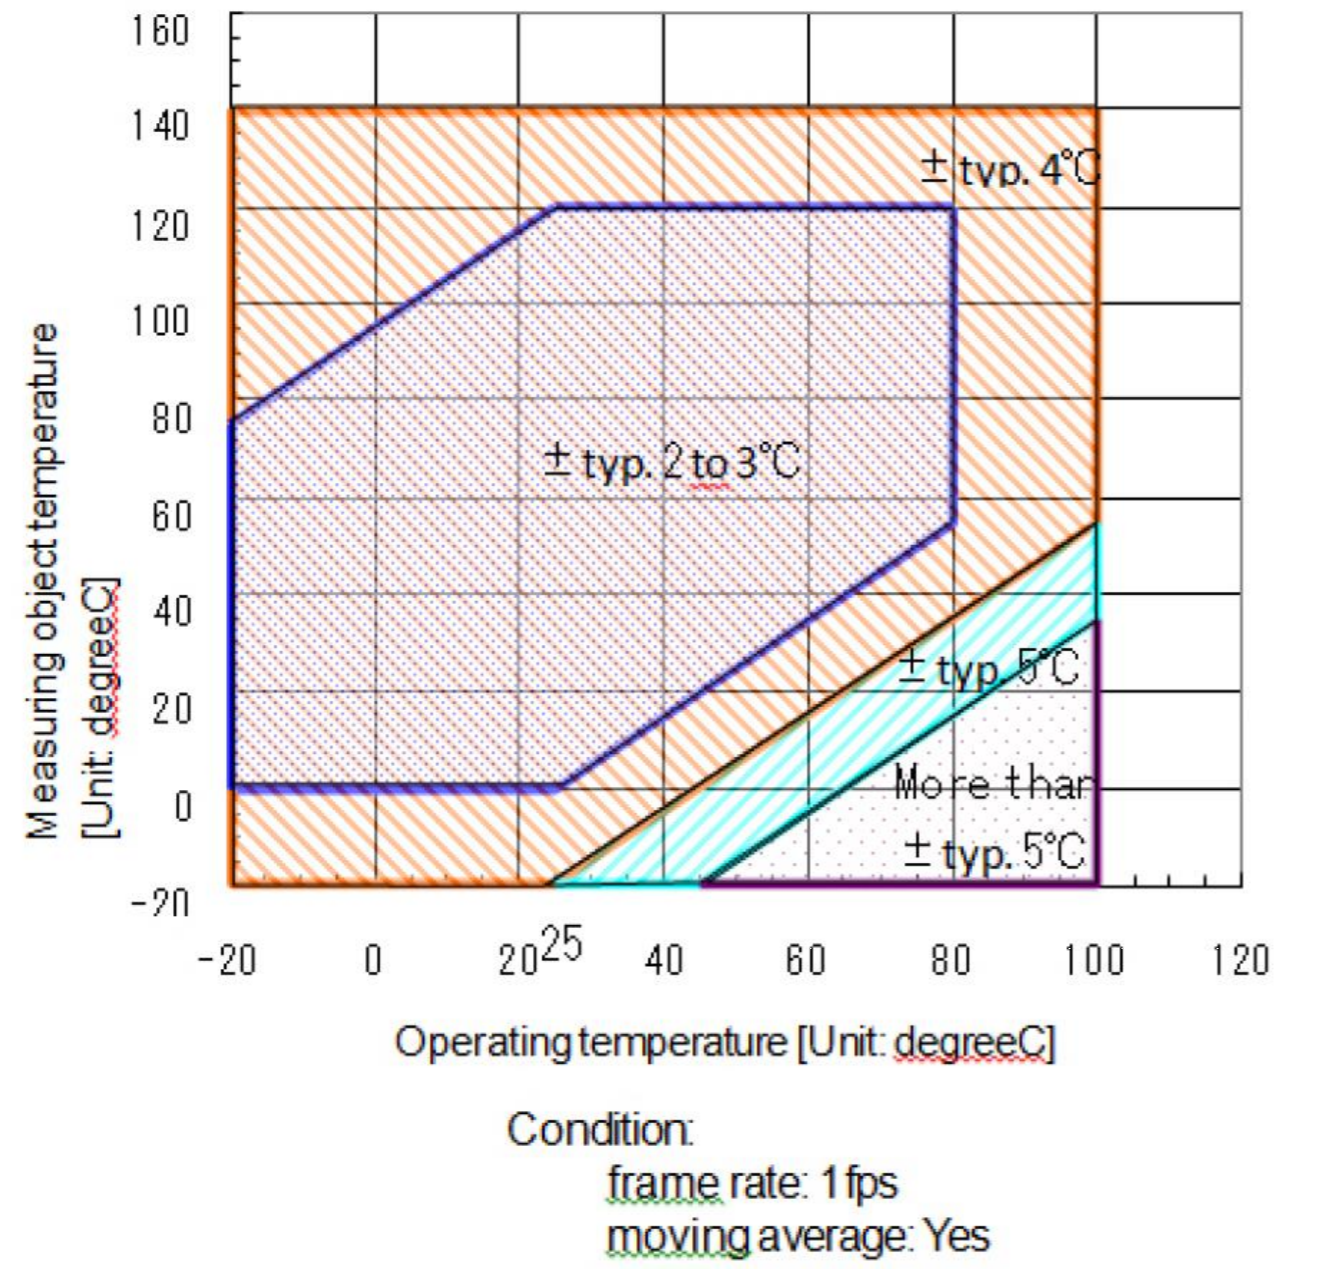
\includegraphics[width=0.8\textwidth]
	{fig/accuracy.PNG}
	\caption[Schema des AMG8834 Sensors]{Schema des AMG8834 Sensors} \protect\cite{AMG8834}
	\label{fig:angleVLP}
\end{figure}
\section{zu messende Objekt}

\begin{figure}[H]
	\centering
	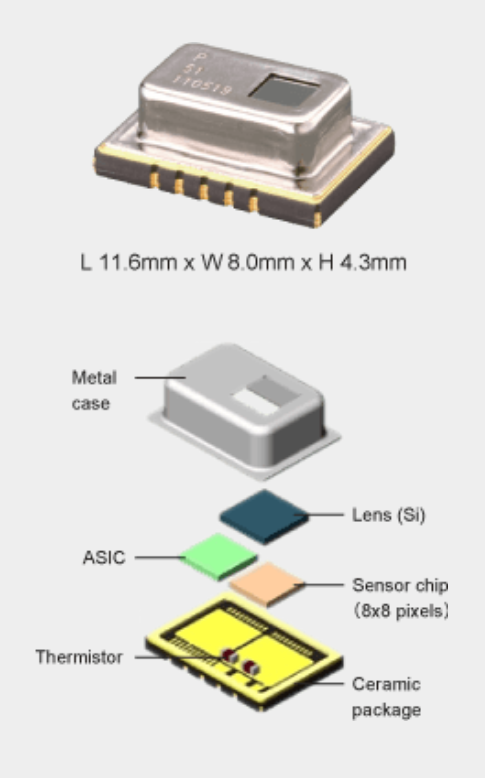
\includegraphics[width=0.5\textwidth]
	{fig/grid_eye_aufbau.PNG}
	\caption[Schema des AMG8834 Sensors]{Schema des AMG8834 Sensors} \protect\cite{AMG8834}
	\label{fig:sens}
\end{figure}

\section{geometrische Aspekte}

\section{zu messende Objekt}


\subsection{Personen}



\subsection{Personenaufzüge}





\section{Störquellen}


\section{verwendete Software}